\scanpage{88}
\mspage{94}

que $X$ est lui aussi asphérique\inserted{, donc $f:X\unsure{\relbar|\to}S$ une $\mathbb D$-équiv.,} (mais les fibres de $X\to S$ ne sont pas $\mathbb D$-asphériques). Cela donne donc un autre contre-exemple au b) de la prop. 6 (p. 84).

Voici la façon la plus économique, je crois, de réaliser la situation que j'ai dite. Topologiquement, je prends \deleted{\unsure{$G$}}

\[
\begin{aligned}
E&=S^2&&\text{sphère euclidienne, sur lequel}\\
&&&\{\pm1\}\text{ opère par antipodisme }x\leftrightarrow-x\\
B&=S^2/\{\pm1\}&&\text{plan projectif réel}\\
&&&(\mathrm{NB}\quad G=\{\pm1\})\\
Z&=S^1&&\text{où $G$ opère comme précédemment}\\
&&&\text{par la \unsure{symétrie|symmétrie}}
\end{aligned}
\]

C'est donc un exemple très proche de celui du début (p. 87), \deleted{mais} où on pourrait aussi considérer la base ($B=S^1$) comme quotient d'un $E$ ($=S^1$) par $G=\{\pm1\}$ opérant librement (par l'antipodisme $z\unsure{\longmapsto|\relbar}-z$ dans $\mathbb C\simeq\mathbb R^2$). Mais dans cet exemple, la base n'était pas $\mathbb D$-asphérique.

La façon la plus économique de réaliser la sphère $S^2$ par un ens ordonné est sans doute par sa décomposition ``globulaire'' par 3 paires de cellules de dim $0,1,2$, donnant l'ens ordonné

\figure{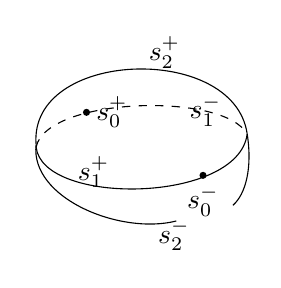
\begin{tikzpicture}[x=1cm,y=1cm]
\draw (0,0.05) .. controls (-.1,1.26) and (2.51,1.35) .. (2.68,.19) .. controls (2.75,-.25) and (2.66,-.58) .. (2.5,-.72);
\draw (0,.05) .. controls (-.08,-.63) and (1.07,-1.10) .. (1.78,-.92);
\draw (0,.02) .. controls (.08,-.73) and (2.56,-.70) .. (2.68,.18);
\draw[dashed] (0,.02) .. controls (.14,.66) and (2.41,.72) .. (2.68,.18);
\fill (.64,.46) circle (.045) node[right] {$s_0^+$};
\fill (2.12,-.34) circle (.045) node[below] {$s_0^-$};
\node at (.73,-.30) {$s_1^+$}; \node at (2.15,.48) {$s_1^-$};
\node at (1.63,1.22) {$s_2^+$}; \node at (1.75,-1.1) {$s_2^-$};
\end{tikzpicture}}

\deleted{\unsure{soit|$Z$}}

\diagram{\begin{tikzcd}[ampersand replacement=\&,row sep=small,column sep=small]
s_2^-\&s_2^+\&\\
s_1^-\arrow[u]\arrow[ur]\&s_1^+\arrow[u]\arrow[ul]\& =\unsure{\overline I|I|\overline J}\\
s_0^-\arrow[u]\arrow[ur]\&s_0^+\arrow[u]\arrow[ul]\&
\end{tikzcd}}

et l'antipodisme échange $s_i^-$ et $s_i^+$, mais le \deleted{groupe} quotient n'est pas ordonné, c'est la catégorie (\deleted{qui} importante pour la théorie des 2-Catégories)

% archive sheet number: 87
